\begin{frame}[fragile]{CNN - Pooling Layers}
\begin{block}{Purpose:}
    \begin{itemize}
        \item Downsample feature maps, reduce spatial dims and parameters, add invariance.
    \end{itemize}
\end{block}

\begin{block}{Types:}
    \begin{itemize}
        \item Max Pooling
        \item Average Pooling
        \item Global Average Pooling
        \item Global Max Pooling
    \end{itemize}
\end{block}

\begin{lstlisting}[language=Python, caption={Code snippet (PyTorch)}, basicstyle=\ttfamily\footnotesize]
import torch.nn as nn

pool = nn.MaxPool2d(kernel_size=2, stride=2)
pooled = pool(x)  # halves H and W
\end{lstlisting}
\end{frame}  

\begin{frame}{CNN - Pooling Layers}
    \begin{figure}
    \centering
    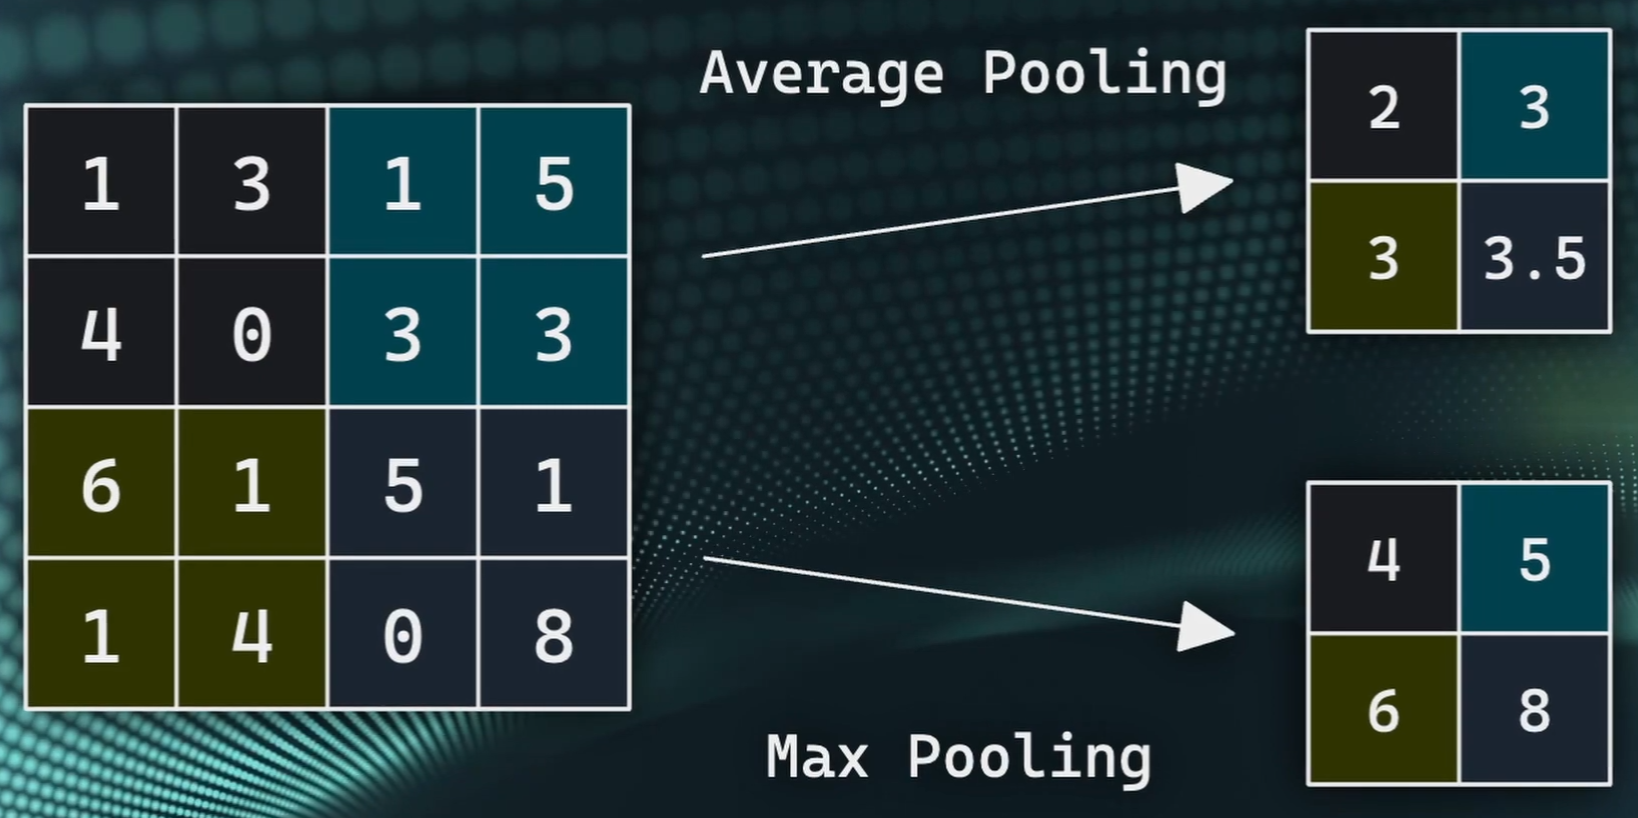
\includegraphics[width=0.95\textwidth,height=0.95\textheight,keepaspectratio]{images/pooling-layer.png}
    \end{figure}
\end{frame}